\section{Background and Motivation}

\subsection{MoE Inference on a Single GPU}
On a single accelerator, expert weights dominate the memory footprint; they comprise roughly 95--96\% of the parameters in the three models studied here~\cite{qwen3technicalreport,qwen3nextmodelcard,abdin2024phi3}. Whether a model fits on-chip depends on how those weights are stored. Expert utilization is also inherently uneven: a small hot set receives a disproportionate share of traffic, so allocating equal fidelity to every expert is rarely cost-effective under a tight memory envelope.

\subsection{Offloading and Prefetching}
\label{sec:background-offload}
A family of systems treats GPU memory as a managed cache and fetches experts on demand~\cite{li2023adaptive,yi2023edgemoe,xue2024moe,eliseev2023fast,hwang2024pre,zhong2024adapmoe,tang2024hobbit,song2024promoe,kong2024swapmoe,shen2025expertflow}. Their opportunity for overlap depends on the size and predictability of the active set. We define instantaneous density as the number of unique selected experts per MoE layer, measured over all nonpadding tokens in a 2,048-token-capped prefill or over the immediately following one-token decode. Each table entry averages five deterministic prompt blocks and all routed layers; batch-$b$ uses the first $b$ prompts of the same 32-prompt block. \autoref{tab:expert_activation_ratio} shows that density rises with batch size: for Qwen3-30B at batch~32, prefill selects 94.0\% of experts and the next decode step selects 26.0\%. Measuring one decode step avoids conflating instantaneous demand with the union accumulated over a long generation. To quantify the transfer consequence in isolation, \autoref{fig:waiting-vs-prompt} replays measured per-layer active sets from a cold cache and serially copies each missed expert from pinned host memory. This microbenchmark reports exposed transfer time for blocking on-demand movement; it is not an end-to-end measurement of an overlapping offload system.

\begin{center}
\colorbox{gray!10}{%
\parbox{0.96\linewidth}{%
\textbf{Observation 1.}
Prefill and larger batches can activate a substantial fraction of the expert pool. A larger instantaneous working set reduces the transfer slack available to an offload cache and increases the cost of misses.}}
\end{center}

\begin{table}[t]
  \centering
  \caption{Mean unique-expert activation ratio (\%) across routed layers and five prompt blocks.}
  \label{tab:expert_activation_ratio}
  \vspace{-0.5em}
  \setlength{\tabcolsep}{3.5pt}
  \begin{tabularx}{\columnwidth}{@{}Xlrrrrrr@{}}
    \toprule
    \textbf{Model} & \textbf{Stage} & \textbf{bs=1} & \textbf{2} & \textbf{4} & \textbf{8} & \textbf{16} & \textbf{32} \\
    \midrule
    Qwen3-30B  & Decode & 6.3 & 7.9 & 11.8 & 16.1 & 20.8 & 26.0 \\
               & Prefill & 59.8 & 70.0 & 82.9 & 89.7 & 92.4 & 94.0 \\
    \midrule
    Qwen3-Next-80B & Decode & 1.9 & 3.7  & 6.7  & 14.9 & 25.4 & 39.2 \\
               & Prefill & 24.6 & 35.3 & 48.8 & 67.1 & 78.9 & 86.2 \\
    \midrule
    Phi-3.5-MoE & Decode & 12.5 & 22.7 & 37.1 & 59.3 & 77.8 & 88.8 \\
                & Prefill & 98.2 & 98.8 & 99.4 & 99.8 & 99.9 & 100.0 \\
    \bottomrule
  \end{tabularx}
\end{table}

\begin{figure}[t]
    \centering
    
\includegraphics[width=0.99\columnwidth]{figures/waiting_latency_vs_prompt_length.pdf}
    \caption{Mean exposed transfer time for cold-cache, trace-driven blocking expert offload on one RTX~A6000 (10 measured trials after two warmups per point).}
    \label{fig:waiting-vs-prompt}
    \vspace{-1.5em}
\end{figure}

\subsection{Static Post-Training Quantization}
\label{sec:background-ptq}

PTQ compresses weights to low bit-widths without retraining. General-purpose schemes such as GPTQ~\cite{frantar2022gptq}, AWQ~\cite{lin2024awq}, SmoothQuant~\cite{xiao2023smoothquant}, and LLM.int8()~\cite{dettmers2022gptint8} have been extended to MoE-specific settings~\cite{kim2023mixturequantizedexpertsmoqe,duanmu2025mxmoe,zhang2025moqe}, where routing imbalance and heterogeneous expert sensitivity motivate per-expert or per-block bit allocation. Once deployed, PTQ incurs no precision-migration traffic. Most pipelines nevertheless fix their precision map during calibration, implicitly treating the resulting expert ranking as stable at inference time.

\begin{figure*}[t]
    \centering
    \begin{minipage}{0.32\linewidth}
        \centering
        \subfloat[WikiText]{%
            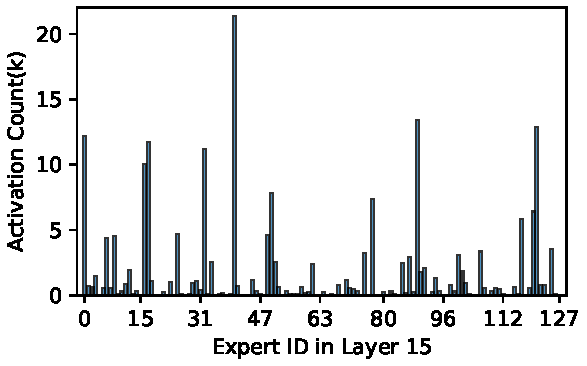
\includegraphics[width=0.95\linewidth]{figures/wikitext_thinking_on_layer_15.pdf}
        }
    \end{minipage}
    \begin{minipage}{0.32\linewidth}
        \centering
        \subfloat[GSM8K]{%
            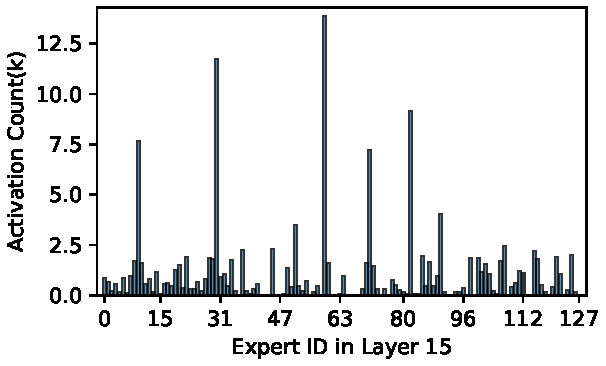
\includegraphics[width=0.95\linewidth]{figures/gsm8k_thinking_off_layer_15.pdf}
        }
    \end{minipage}
    \begin{minipage}{0.32\linewidth}
        \centering
        \subfloat[HumanEval]{%
            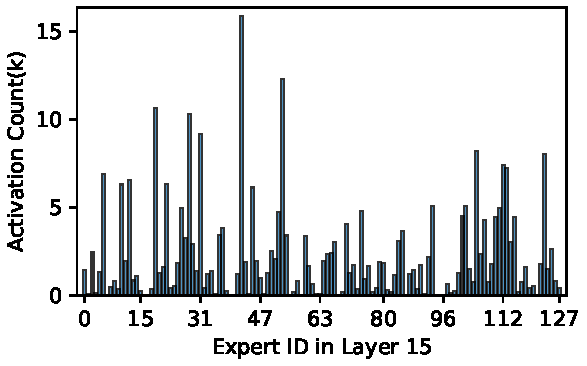
\includegraphics[width=0.95\linewidth]{figures/humaneval_thinking_on_layer_15.pdf}
        }
    \end{minipage}
    \caption{Selected token--expert dispatch counts at Layer~15 of Qwen3-MoE-30B under the full pinned WikiText, GSM8K, and HumanEval workloads. The scheduler is frozen with all experts at INT4; the top-10 most frequently selected experts are entirely disjoint across text, math, and code tasks.}
    \label{fig:expert-active}
    \vspace{-1.0em}
\end{figure*}

That assumption is brittle for MoE. Expert utilization is heavy-tailed and the identity of hot experts shifts across workloads (\autoref{fig:expert-active}). We count every selected top-$k$ token--expert dispatch, rather than thresholding router probabilities, and reset the counter between the three full evaluation workloads. Under this pinned protocol, the top-10 most frequently selected experts for text, math, and code are entirely disjoint.

\begin{center}
\colorbox{gray!10}{%
\parbox{0.96\linewidth}{%
\textbf{Observation 2.}
MoE expert usage is heavy-tailed and workload-dependent: a small set receives much of the traffic, but its membership changes across tasks. A precision map optimized for one routing distribution can therefore become stale.}}
\end{center}

\subsection{Motivation and Challenges for Online Precision Control}
\label{sec:background-motivation}

The observations above suggest adapting expert precision online under a strict GPU budget. A natural concern is whether such adaptation destabilizes quality. We concatenate the pinned WikiText-2 test split and measure perplexity over at most 128 exact 2,048-token windows while increasing the fraction of low-precision experts per layer. We obtain one expert ranking from the independent calibration corpus, freeze online reassignment, and demote an exact suffix of that same ranking at every point; thus, the sweep isolates the precision quota rather than conflating it with scheduler adaptation. As \autoref{fig:ppl} shows, when demotion targets infrequently activated experts first, perplexity rises smoothly.

\begin{center}
\colorbox{gray!10}{%
\parbox{0.96\linewidth}{%
\textbf{Observation 3.}
When demotion follows a fixed cold-to-hot ranking, perplexity changes smoothly with the low-precision quota. Expert precision therefore exposes a controllable quality--memory tradeoff.}}
\end{center}

\begin{figure}[t]
    \centering
    \begin{minipage}{0.46\linewidth}
        \centering
        \subfloat[Qwen3-30B]{%
            
\includegraphics[width=0.95\linewidth]{figures/wiki_ppl_qwen30b.pdf}
        }
    \end{minipage}
    \begin{minipage}{0.46\linewidth}
        \centering
        \subfloat[Qwen3-Next-80B]{%
            
\includegraphics[width=0.95\linewidth]{figures/wiki_ppl_qwen80b.pdf}
        }
    \end{minipage}
    \caption{Perplexity vs.\ low-precision expert ratio (Qwen3-30B: FP16 vs.\ INT4; Qwen3-Next-80B: INT4 vs.\ INT2).}
    \label{fig:ppl}
    \vspace{-1em}
\end{figure}

Realizing this tradeoff at runtime, however, requires satisfying three constraints:
\begin{itemize}[leftmargin=1.5em, itemsep=1pt, topsep=2pt]
    \item \textbf{Hard expert-budget invariance.} Precision changes alter the resident footprint. The runtime must never exceed the device envelope allocated to expert residency and transitions; otherwise out-of-memory failures or forced evictions cascade into instability. The deployment must separately size KV-cache and activation reserves for its supported request shape.
    \item \textbf{Critical-path isolation.} Precision transitions involve heavyweight device transfers that must not stall the forward pass.
    \item \textbf{Tail-latency robustness.} Naive reallocation can thrash when routing scores fluctuate, amplifying migration traffic and widening P99 latency.
\end{itemize}
